\documentclass[../main]{subfiles}
\begin{document}
\section{Introduction}
%\section{Problem Description}
%Many State of the art models today have a large memory footprint, therefore with the advent of various devices with diif 

Convolutional Neural Networks have made monumental progress in image classification, object detection and various other applications.
While these carefully designed deep convolutional networks continue to increase performance for various tasks, they continue to become deeper and larger \citep{szegedy2017inception,real2018regularized,hu2017squeeze}, while becoming slower and requiring more computational resources both in terms of memory footprint and as well as inference time.
Due to this increased computational and memory demands it becomes difficult to deploy models to mobile or embedded devices where memory and computational resources are at a premium.
Furthermore data on various devices are distributed differently and we would essentially want best performance on user specific data samples and want our models to be tailored specifically for different users depending upon the data distribution.
We perform experiments on subsets of the dataset, which have been considered as proxy for the real world scenario where different users have different data.
There is a need to personalize the model, specifically tailoring it for a particular user.

Recently there has been much research on reducing the depth of the networks \citep{iandola2016squeezenet} and utilizing less expensive operation, such as depth-wise convolution \citep{howard2017mobilenets} and group convolution \citep{DBLP:journals/corr/ZhangZLS17} but all these require manual effort to design network which are efficient for mobile devices.
This is a tedious and time consuming task.
Furthermore, these architectures need to have the right trade-off between performance and efficiency.
In this paper we propose an automated system to compress the state of the art neural network architectures used as feature extractors.
Current techniques for compressing state of the art models utilize Knowledge Distillation, which is essentially mapping a large (teacher) network to a smaller (student) network using techniques such as soft output matching or uncertainty modelling.
The problem with Knowledge Distillation is that it still requires us to carefully handcraft architectures for the student network.
Handcrafting architectures is a trial and error process which is tedious, time consuming and can be highly sub-optimal.
Further, hand-designing student architectures for different users or groups depending on their data is infeasible for large user bases.
Clearly, there is a need for a principled way to identify good student architectures.

Our approach builds upon system developed by \citet{ashok2017n2n} which utilizes reinforcement learning (RL) to obtain the optimal student architecture from a state of the art teacher model.
We incorporate the inference latency of the produced student in addition to accuracy and compression and pose it as a multi-objective optimization problem.
Further, we propose a method to transfer the neural architecture learned from one user dataset to another.
This allows us to further reduce the time to find good compressed architectures \wrt{} different users.
We validate the methods with experiments.
We test on two different families, \viz~ResNet and VGGnet and \wrt{} data subsets of CIFAR-10, CIFAR-100 and Caltech-256 datasets.
Our contributions are enumerated below:
\begin{itemize}
	\item For a RL based multi-objective neural architecture search approach, we design the reward functions with user definable performance thresholds for accuracy, compression ratio and inference latency, as inputs to the search algorithm.
	The user definable thresholds allow us to control the trade-off between the metrics for different deployment targets.
	\item We demonstrate that the optimal architectures for different data subsets are different.
	This is evidence towards model personalization.
	\item We introduce a regime of utilizing the original model outputs and target while training the  to outperform previously published work by \citet{ashok2017n2n,hinton2015distilling}.
	\item We show that the neural architecture search result for one data subset transfers to other data subsets.
	This leads to a reduction in the time needed to find good personalized architectures across large user bases.
	We emphasize that this compression policy transfer is across data subsets and is completely different from that explored in \citet{ashok2017n2n}.
	The latter work provides evidence that the compression policy transfers between model instances within the same architecture family (\eg~policy learnt on ResNet-18 transfers to ResNet-34).
\end{itemize}

\begin{figure}
  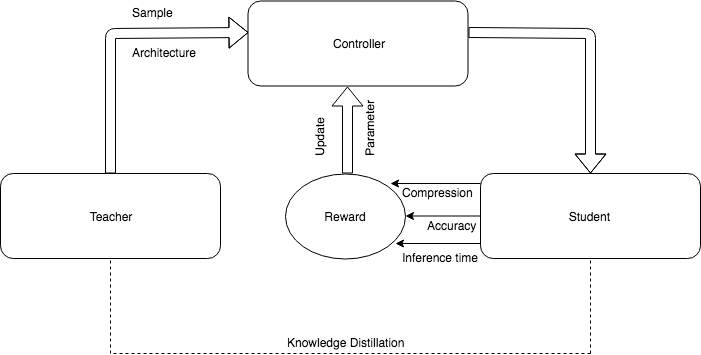
\includegraphics[width=\linewidth]{system}
  \caption{A recurrent controller which sample an architecture $p$ from the teacher model to produce a smaller student model.
  Combination of Accuracy $a$, Compression $c$ and Inference time $l$ is considered as a metric to scrutinize a generated architecture.
  This reward is then used to update the parameters of the recurrent controller.}
  \label{fig:boat1}
\end{figure}



%\subsection{Contributions}
%Today, the researchers are working on developing hand-crafted deep convolutional networks, these neural networks are large in size and can’t be deployed on small devices like mobile or IOT device.
%Many compression techniques are used to reduce their sizes as Knowledge distillation, Pruning, Quantization.
%The problem with the existing methods are two folds handcrafting deep neural models is a tedious job and requires 
%\begin{itemize}
%\item A more sophisticated approach for doing that was introduced in [1] called N2N, which is a reinforcement learning based approach which performs optimal architectural search based on the knowledge distilled from a larger teacher model.
%N2N doesn't take into account the inference time for the compressed model.
%\item Inference time is one of the main performance indicators for on-device machine learning.
%We want to model a more real world scenario in which we consider the inference time for the model, while preserving the accuracy and achieving reasonable compression.
%We have analyzed  reward functions taking into account the accuracy, compression ratio and the inference time to arrive on an optimal architecture, which was not previously possible through hand crafted architecture, which require large human effort and resources.
%The relative contribution of accuracy and the compression ratios have been studied and modified to obtain optimal results.
%We have demonstrated through our experiments the enhancement in the model’s optimum values especially the inference time.
%\item On device machine learning is to enhance the personalisation aspect which refers to performing better on user specific data subset,  N2N compression technique distills the knowledge from the teacher model to the student model and based upon the soft and hard loss functions arrives at the optimal architecture.
%A policy to compress is learnt in the process which decides which layer is to be removed depending upon the dataset.
%\item We have analyzed the re-usability of a policy trained on one dataset and it transferability of the same policy across dataset.
%Our policy transfer experiments demonstrate its effectiveness in speeding up the architecture search and reaching optimal compression, in comparison to training the policy from scratch.
%\item We demonstrate the effectiveness of our approach and inferences over several network architectures and several visual learning tasks (MNIST, CIFAR-10, CIFAR-100).
%\item We also demonstrate that the compression policies exhibit generalization across networks with similar architectures.
%In particular, we use a policy trained on a ResNet-18 model on a ResNet-34 model and show that it greatly accelerates the reinforcement learning process.
%\end{itemize}


\bibsubfile
{plainnat}
{bibs/sub}

\end{document}
